\documentclass[tikz,border=2pt]{standalone}
\usepackage{tikz}
\usetikzlibrary{arrows.meta, bending,calc}

\begin{document}
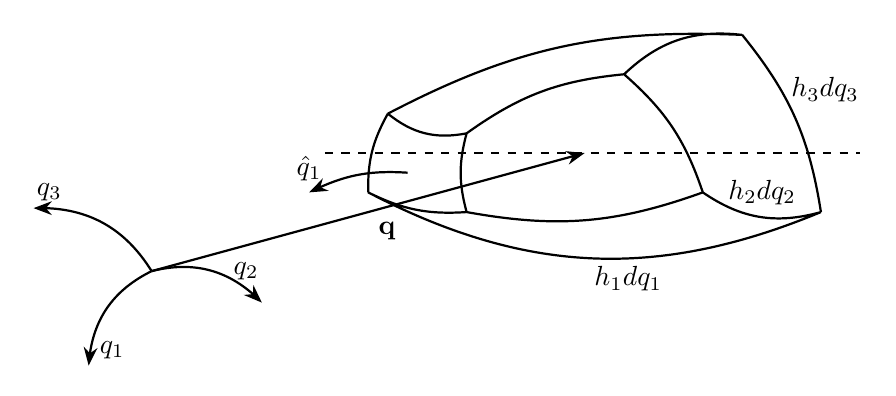
\begin{tikzpicture}[>=Stealth]

% --- Coordinate System Axes (Bottom Left) ---
\coordinate (O) at (0,0);
\draw[->, thick, bend right=30] (O) to (-0.8,-1.2);
\node at (-0.5,-1) {$q_1$};
\draw[->, thick, bend left=30] (O) to (1.4,-0.4);
\node at (1.2,0) {$q_2$};
\draw[->, thick, bend right=30] (O) to (-1.5,0.8);
\node at (-1.3,1) {$q_3$};

% --- Volume Element ---
\coordinate (A1) at (2.75,1);
\coordinate (A2) at (3,2);
\coordinate (A3) at (4,1.75);
\coordinate (A4) at (4,0.75);
\coordinate (B1) at (7,1);
\coordinate (B2) at (6,2.5);
\coordinate (B3) at (7.5,3);
\coordinate (B4) at (8.5,0.75);

\draw[thick] (A1) to[bend left=15] (A2)
(A2) to[bend right=25] (A3)
(A3) to[bend right=15] (A4)
(A4) to[bend left=15] (A1)
(B1) to[bend right=15] (B2)
(B2) to[bend left=25] (B3)
(B3) to[bend left=15] (B4)
(B4) to[bend left=25] (B1)
(A2) to[bend left=15] (B3)
(A3) to[bend left=15] (B2)
(A4) to[bend right=15] (B1)
(A1) to[bend right=25] (B4);


% --- Vectors and Lines ---
\draw[->, thick] (O) -- node[below right] {$\mathbf{q}$} (5.5, 1.5); % q vector to center
\draw[dashed] (2.2, 1.5) -- (9, 1.5); % Centerline
\draw[->, thick] (3.25,1.25) to[bend right=15]  (2,1); 
\node at (2,1.3) {$\hat{q}_1$};

% Labels 
\node[right] at (8, 2.3) {$h_3 dq_3$};
\node[right] at (7.2, 1) {$h_2 dq_2$};
\node[right] at (5.5, -0.1) {$h_1 dq_1$};

\end{tikzpicture}
\end{document}